\documentclass[twoside,11pt]{article}
\usepackage[margin=3cm]{geometry}


\usepackage{amsmath}
\usepackage{amssymb}
\usepackage{bm}
\usepackage{natbib}
%\usepackage[style=numeric,natbib=true]{biblatex}


\bibliographystyle{chicago}

\RequirePackage[colorlinks=true,citecolor=blue,allbordercolors={1 1 1}]{hyperref}
%\addbibresource{bibliography.bib}
%\bibliography{bibliography}
\usepackage{todonotes} 

\usepackage{subfig}

\usetikzlibrary{bayesnet,calc,angles,quotes}
\usepackage{tikz-3dplot}
\usetikzlibrary{decorations.pathreplacing}
\usepackage[utf8]{inputenc}

\usepackage{amsthm}
\newtheorem{corollary}{Corollary}
\newtheorem{theorem}{Theorem}
\newtheorem{proposition}{Proposition}
\newtheorem{claim}{Claim}
\newtheorem{definition}{Definition}
\newtheorem{lemma}{Lemma}
\newtheorem{assumption}{Assumption}
\newtheorem{problem}{Problem}
\newtheorem{example}{Example}


%\DeclareMathOperator{\dim}{\mathrm{dim}}
\DeclareMathOperator{\Tr}{Tr}
\DeclareMathOperator{\St}{St}
\DeclareMathOperator{\Sp}{\mathrm{Sp}}
\DeclareMathOperator{\Diam}{\mathrm{Diam}}
\DeclareMathOperator{\Diag}{\mathrm{Diag}}
\DeclareMathOperator{\rank}{\mathrm{rk}}
\DeclareMathOperator{\Det}{Det}
\DeclareMathOperator{\Vol}{Vol}
\DeclareMathOperator{\Adj}{Adj}
\DeclareMathOperator{\Span}{\mathrm{Span}}
\DeclareMathOperator{\Conf}{\mathrm{Conf}}
\DeclareMathOperator{\Fr}{\mathrm{Fr}}
\DeclareMathOperator{\DPP}{\mathrm{DPP}}
\DeclareMathOperator{\Cor}{\mathrm{Cor}}
\DeclareMathOperator{\VS}{\mathrm{VS}}
\DeclareMathOperator{\HS}{\mathrm{HS}}
\DeclareMathOperator{\OP}{\mathrm{op}}
\DeclareMathOperator{\eff}{\mathrm{eff}}
\DeclareMathOperator{\Tran}{\intercal}
\newcommand{\dataset}{{\cal D}}
\newcommand{\fracpartial}[2]{\frac{\partial #1}{\partial  #2}}
\DeclareMathOperator{\EX}{\mathbb{E}}
\DeclareMathOperator{\Var}{\mathbb{V}}
\DeclareMathOperator{\Prb}{\mathbb{P}}
\DeclareMathOperator*{\argmax}{arg\,max}
\DeclareMathOperator*{\argmin}{arg\,min}
\DeclareMathOperator*{\KDPP}{\mathfrak{K}}

\DeclareMathOperator{\F}{\mathcal{F}}
\DeclareMathOperator{\X}{\mathcal{X}}
% Expectation symbol


\newcommand{\ab}[1]{\textcolor{red}{#1}}
\newcommand{\pc}[1]{\textcolor{blue}{#1}}
\newcommand{\rb}[1]{\textcolor{magenta}{#1}}


\usepackage{bbold}
% Definitions of handy macros can go here



% Expectation symbol

%\DeclareRobustCommand{\bbone}{\text{\usefont{U}{bbold}{m}{n}1}}


% Heading arguments are {volume}{year}{pages}{date submitted}{date published}{paper id}{author-full-names}



% Short headings should be running head and authors last names

%\firstpageno{1}

\begin{document}

\title{Thesis manuscript}


\author{Ayoub Belhadji} %if necessary, replace with your course title
 
\maketitle
%\author{\name Authors}

%\editor{Editors}

%\maketitle

%\begin{abstract}%   <- trailing '%' for backward compatibility of .sty file
%aaa
%\end{abstract}



\newpage
%\section{Introduction en français}
\section{Introduction}
\subsection{Sensing on budget} 
(3 pages)
\subsection{Design problems in applied mathematics}
(3-6 pages)
\subsection{Mathematical framework: Determinantal point processes}
(7-10 pages)

\subsection{The layout}
(2 pages)
\section{The column subset selection problem}\label{chapter:cssp}
\subsection{Related work}
\subsection{The proposed algorithm}
% \subsubsection{The projection DPPs}
% \subsubsection{The intuitions}
\subsection{Principal angles between subspaces}
\subsection{Main results}
\subsubsection{Low rank approximations}
\subsubsection{Linear regression}
\subsection{Numerical experiments}
\subsection{Discussion} (5-6 pages)
\begin{itemize}
\item Probabilistic inequalities
\item A consequence for Rank Revealing QRs
\item A consequence for graph signal reconstruction
\item Connexions with optimal design problems
\item The difference between sparse PCA and CSSP
\item The approximation of the volume by random projections 
\item The limitations 
\end{itemize}
\subsection{Prologue: the infinite column subset selection problem} (1-2 pages)

\clearpage
\section{Kernel quadrature using DPPs}
\subsection{Numerical integration problems}

\subsection{Related work}
The purpose of this section is to motivate the theoretical analysis of a class of quadratures based on projection DPPs that is naturally defined in the RKHS framework. The merit of this class of quadratures is its universality and applicability to a variety of settings. An exhaustive review of existing results on quadratures is outside the scope of this manuscript; nevertheless, it turns out that many landmark results on the field are connected to projection DPPs. For this reason, we review these classic results in the following.



% More importantly, the connexions between projection DPPs and existing work on quadratures is highlighted. 


% For this purpose, we review existing results on quadratures 


\subsubsection{Quadratures on the real line}
We start by a brief review on quadratures on the real line.
\paragraph{Newton-Cotes quadrature}
The approximation of the integral of a function $f$ on some interval $[a,b]$ using some evaluations of $f$ can be tracked to the work of Newton. The idea of the eponymous quadrature is to consider a set of nodes $\bm{x} = \{x_{1}, \dots , x_{N} \} \subset \X^{N}$, and the corresponding interpolating polynomial of degree $N-1$:
\begin{equation}
p_{N-1}(X) = \sum\limits_{n \in [N]} f(x_{n}) \ell_{n,\bm{x}}(X),
\end{equation}
where $\ell_{n,\bm{x}}$ is defined by
\begin{equation}
\ell_{n,\bm{x}}(X) = \frac{\prod\limits_{m \in [N], m \neq n }(X-x_{m})}{\prod\limits_{m \in [N], m \neq n }(x_{n}-x_{m})}.
\end{equation}
The idea of Newton was to consider the approximation
\begin{align}\label{eq:Newton_approx}
\int_{a}^{b}f(t)\mathrm{d}t & \approx \int_{a}^{b}p_{N-1}(t)\mathrm{d}t  \\
& =  \sum\limits_{n \in [N]}f(x_{n}) \int_{a}^{b} \ell_{n,\bm{x}}(t) \mathrm{d}t.\\
& :=  \sum\limits_{n \in [N]}f(x_{n}) w_{n} .
\end{align}
The approximation \eqref{eq:Newton_approx} is exact if $f$ is a polynomial of order less than $N-1$. The scalars $w_{n}$ are called Cotes numbers
\paragraph{Gaussian quadratures}
As we have seen previously, the Newton-Cotes quadrature is exact for polynomials of order less than $N-1$. Gauss interested in the maximal order of exactness that could be achieved using the Newton-Cotes quadrature. This order depends on the design of nodes $\bm{x}$ and is defined by 

\begin{equation}
M(\bm{x}) = \sup \{ m \in \mathbb{N}, \: \int_{a}^{b} t^{m} \mathrm{d}t = \sum\limits_{n \in [N]} w_{n}x_{n}^{m} \}.
\end{equation}


%  that the $M(\bm{x}) \geq N-1$ for any proper design $\bm{x}$

% Gauss dealed with the maximal order of exactness in the Newton-Cotes quadrature:\\

% \emph{For a fixed value $N$, what is the maximal order $M(\bm{x})$ of polynomials such that the approximation \eqref{eq:Newton_approx} is exact?}

Gauss proved that there exists a design $\bm{x}_{G}$ such that $M(\bm{x}_{G}) = 2N-1$, and that this order is maximal among all the possible designs. The proof of Gauss is based on arguments from continued fractions theory.
% In particul there exists a remarkable design of nodes that achieves a higher degree of exactness: the approximation \eqref{eq:Newton_approx} is exact if $f$ is a polynomial of order less than $2N-1$.

An alternative proof was given by Jacobi in [????], where he proved the existence of such a design, $\bm{x}_{G}$, that we call the Gauss nodes, using simple arguments of polynomial divisibility. Indeed, Jacobi shows that for any integer $N' \in [N]$, the Newton-Cotes quadrature has the maximal degree of exactness $M(\bm{x}) = N-1+N'$ if and only if for every polynomial $p$ of order less than $N'-1$:

\begin{equation}
\int_{a}^{b} p(t) \pi_{\bm{x}}(t) \mathrm{d}t = 0,
\end{equation}
where $\pi_{\bm{x}}$ is the polynomial
\begin{equation}
\pi_{\bm{x}}(X) = \prod\limits_{n \in [N]}(X-x_{n}).
\end{equation}
The case $N' = N$ leads to the Gauss formula of maximal degree of exactness $2N-1$. More importantly, this characterization of Gauss nodes, proved by Jacobi, highlights the importance of orthogonality between polynomials: the Gauss nodes are the roots of a polynomial of degree $N$ that is orthogonal to all polynomials of degree less than $N-1$. The corresponding nodes polynomials $\pi_{\bm{x}}$ are nothing else but the scaled Legendre polynomials.

The notion of orthogonality between polynomials was pushed further by considering quadrature problems with respect to weighted measures: $\mathrm{d}\omega = w(t) \mathrm{d} t$.

\begin{equation}
\int_{a}^{b}f(t)w(t)\mathrm{d}t \approx \sum\limits_{n \in [N]} w_{n}f(x_{n}).
\end{equation}

% In general, 




\subsubsection{Quasi-Monte Carlo methods}
The weights of a Quasi Monte Carlo quadrature are uniform $\displaystyle w_{i} = \frac{1}{N}$, while the nodes, defined on $\mathcal{X} = [0,1]^{D}$, are deterministic, and "well-spread", such that the quadrature error is small for a certain class of functions. 
\clearpage




As we have seen previously, several quadrature rules are known for functions defined on the real line. The situation is far more complicated for integration problems in high-dimension. For instance, the uniform grid suffers from the "curse of the dimension". To precise the meaning of the curse in this context, we review some notions on low discrepancy sequences also known as quasi-Monte Carlo methods.


 
\paragraph{The discrepancy functions}

\begin{figure}
\centering
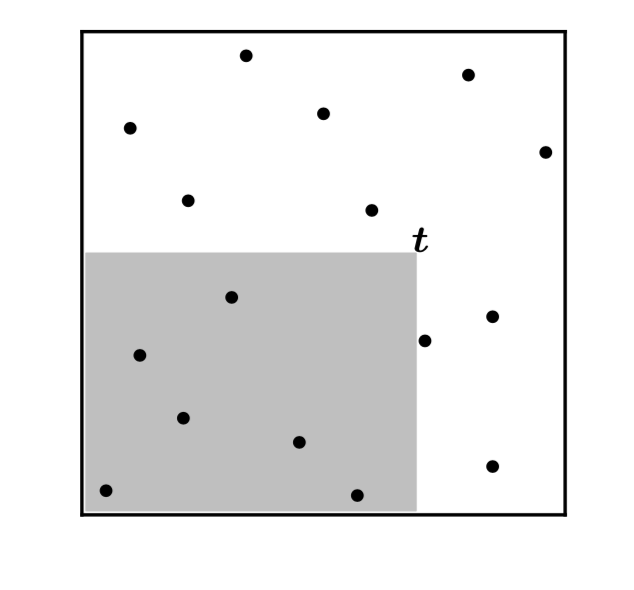
\includegraphics[width= 0.35\textwidth]{img/discrepancy/local_disc.png}
\caption{\label{fig:local_discrepancy}}
\end{figure}

 A discrepancy function of a design $\bm{x} \subset \X^{N}$ quantifies the "spread" of the nodes of $\bm{x}$. It is defined with respect to a set of test sets $\mathcal{S}$.





  For example, in $\mathcal{X} = [0,1]^{d}$, a typical choice of $\mathcal{S}$ is the set of the Cartesian products $[\bm{0},\bm{u}] = \prod_{\delta \in [d]}[0,u_{\delta}]$ with $\bm{u} \in \mathcal{X}$. In this case, the local discrepancy is defined for all $\bm{u} \in \X$ by 
\begin{equation}\label{def:discrepancy}
\Delta_{\bm{x}}(\bm{u}) = \frac{1}{N}\sum\limits_{n \in [N]} \mathbb{1}_{[\bm{0},\bm{u}]}(x_{n}) - \prod\limits_{\delta \in [d]}u_{\delta}.
\end{equation}  
The term $\displaystyle \frac{1}{N}\sum\limits_{n \in [N]} \mathbb{1}_{[\bm{0},\bm{u}]}(x_{n})$ in \eqref{def:discrepancy} counts the number of the nodes $x_{n}$ that falls into $[\bm{0},\bm{u}]$ divided by the total number $N$; while the second term $\displaystyle  \prod\limits_{\delta \in [d]}u_{\delta}$ measures the volume of $[\bm{0},\bm{u}]$: $\Delta_{\bm{x}}$ measures the difference between the relative number of points that belongs to the interval $[0,\bm{u}]$ and its volume. A design of nodes $\bm{x}$ would be "well-spread" if the discrepancy function $\Delta_{\bm{x}}$ is low in $\X$. A way to quantify this "spreadness" is by taking the $\|.\|_{p}$ norm of the local discrepancy function on $\X$. Indeed, for $p \in [1,\infty]$, $\Delta_{\bm{x}} \in \mathbb{L}_{p}(\mathbb{R}^{d})$ because $[0,1]^{d}$ is a compact set of $\mathbb{R}^{d}$; and the $\mathbb{L}_{p}$-discrepancy of $\bm{x}$ is defined by 
\begin{equation}
\Delta_{p}(\bm{x}) = \bigg(\int_{[0,1]^{d}}\Delta_{\bm{x}}(\bm{u})^{p} \mathrm{d}\bm{u}\bigg)^{1/p}.
\end{equation}
In particular, the $\|.\|_{\infty}$ norm of the local discrepancy is called the \emph{star-discrepancy} and it is denoted $\Delta_{*}(\bm{x})$.

Figure~\ref{fig:local_discrepancy} illustrates the concept of local discrepancy on $[0,1]^{2}$: the two hypercubes $[\bm{0},\bm{u}_{1}]$ and $[\bm{0},\bm{u}_{2}]$ have the same volume, yet the corresponding local discrepancies with respect to the design $\bm{x}$ are not equal as $[\bm{0},\bm{u}_{1}]$ contains more nodes from the design than $[\bm{0},\bm{u}_{2}]$.

Another example is the hypersphere $\X = \mathbb{S}^{d-1}$, where commonly considered test sets are the spherical caps defined by
\begin{equation}
C(t,\bm{u}) = \{ \bm{v} \in \mathbb{S}^{d-1}, \: \langle \bm{v}, \bm{u} \rangle \geq t\},
\end{equation}
% where $t \in [-1,1]$ and $\bm{u} \in \mathbb{S}^{d-1}$ 
\paragraph{Koksma-Hlawka inequalities}
The discrepancy functions for a design $\bm{x}$ play an important role in the quantification of the integration error based on $\bm{x}$. Indeed, consider the quadrature:
\begin{equation}
\frac{1}{N} \sum\limits_{n \in [N]}  f(x_{n}),
\end{equation}
as an approximation of $\displaystyle \int_{[0,1]^{d}} f(\bm{u}) \mathrm{d}\bm{u}$. The relationship between the discrepancy functions and the integration error clear up considering the Koksma-Hlawka inequalities.

\begin{theorem}\label{thm:KH_ineq}
Let $p,q \in [1,+\infty]$, such that $1/p+1/q = 1$. Consider $f \in \mathbb{L}_{q}([0,1]^{d})$. Then 
\begin{equation}\label{eq:KH_ineq}
\bigg| \int_{[0,1]^{d}} f(\bm{u}) \mathrm{d}\bm{u} - \frac{1}{N} \sum\limits_{n \in [N]}  f(x_{n})\bigg| \leq \Delta_{p}(\bm{x}) \|\frac{\partial^{d} f}{\partial \bm{u}}\|_{q}.
\end{equation}
\end{theorem}
The Koksma-Hlawka inequalities gives a decoupled upper bound on the integration error: the $\mathbb{L}_{p}([0,1]^{d})$ discrepancy of the design $\bm{x}$ does not depend on $f$ and the $q$ variation of the function $f$ does not depend on the design $\bm{x}$. This decoupling allows to focus only on the discrepancy of the design. 

Looking for designs having the lowest discrepancy was a topic of intense research.  A very brief review of this line of research is provided in the following paragraph. 
\paragraph{Low discrepancy sequences}



\begin{figure}
\centering
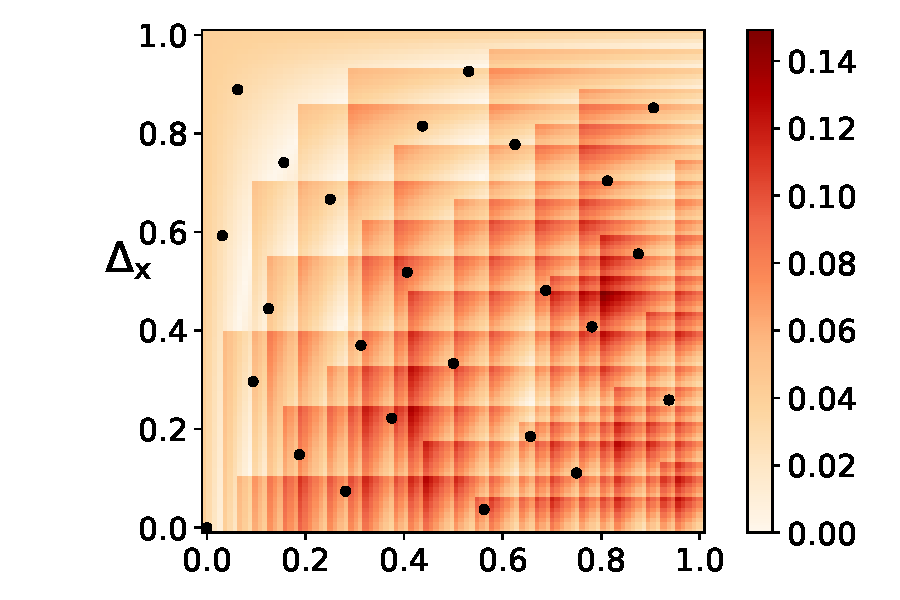
\includegraphics[width= 0.32\textwidth]{img/discrepancy/local_discrepancy_halton_N_25.pdf}~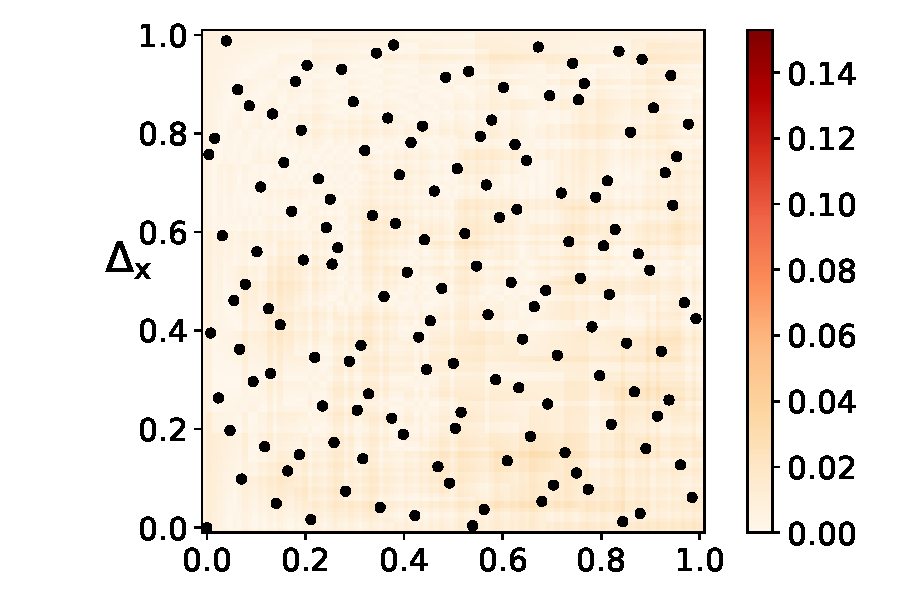
\includegraphics[width= 0.32\textwidth]{img/discrepancy/local_discrepancy_halton_N_144.pdf}
~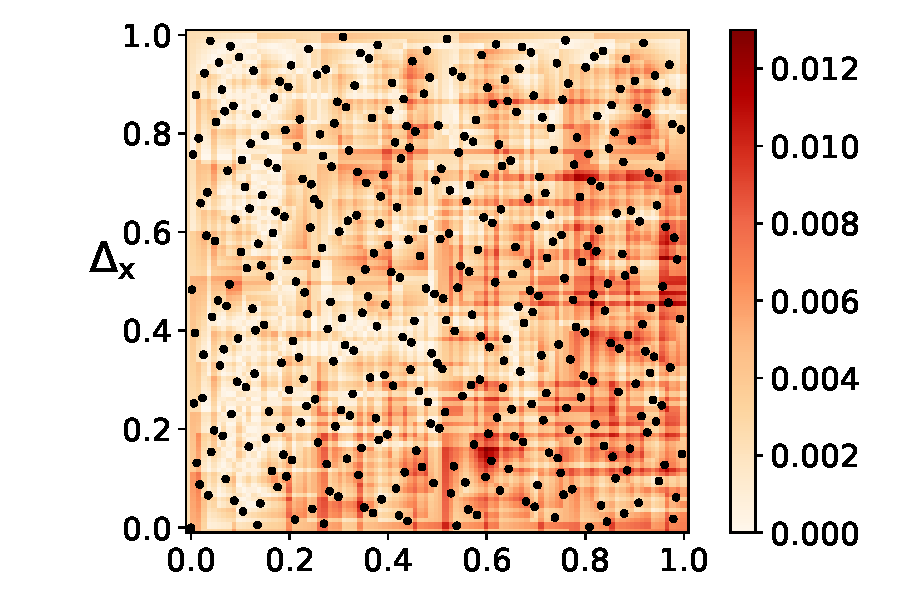
\includegraphics[width= 0.32\textwidth]{img/discrepancy/local_discrepancy_halton_N_400.pdf}\\
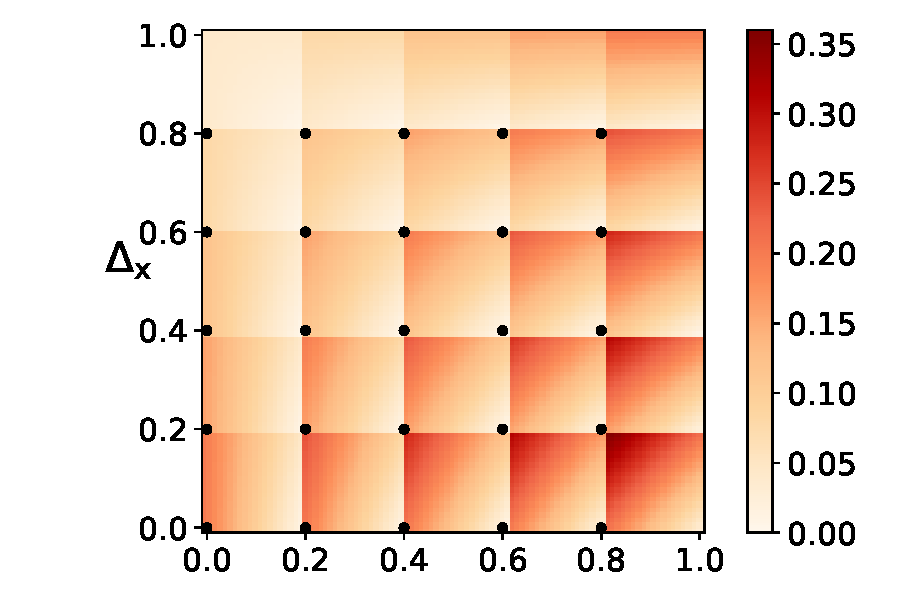
\includegraphics[width= 0.32\textwidth]{img/discrepancy/local_discrepancy_uniform_grid_N_25.pdf}~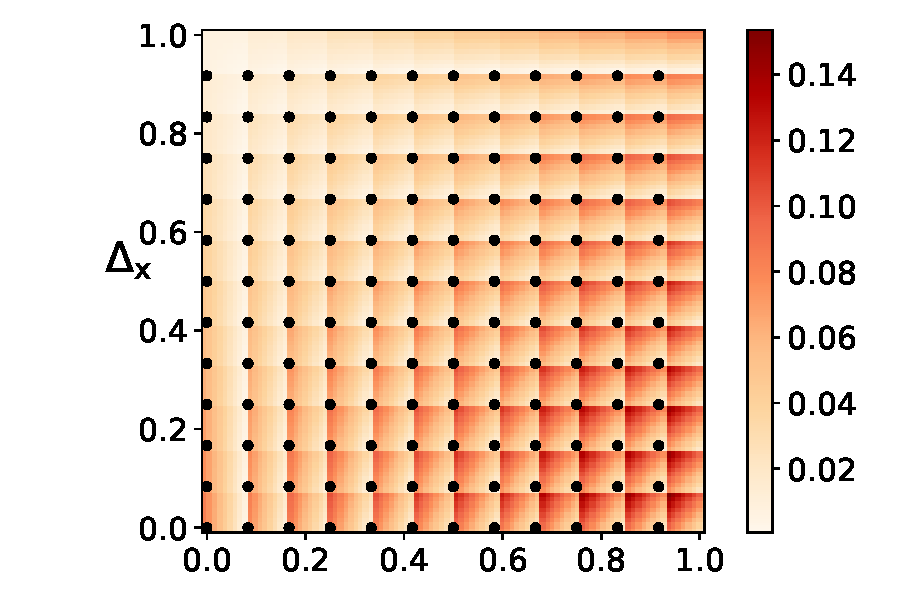
\includegraphics[width= 0.32\textwidth]{img/discrepancy/local_discrepancy_uniform_grid_N_144.pdf}
~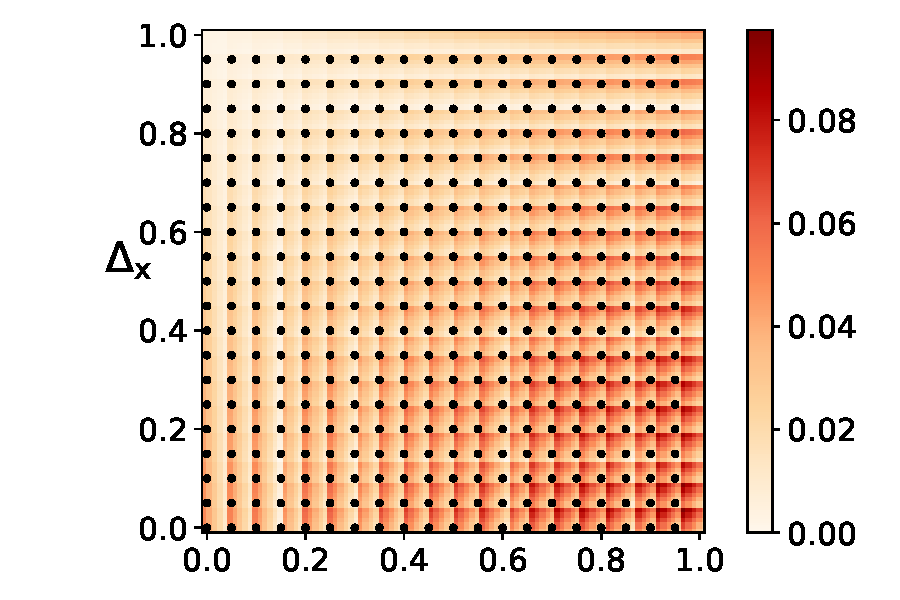
\includegraphics[width= 0.32\textwidth]{img/discrepancy/local_discrepancy_uniform_grid_N_400.pdf}
\caption{The local discrepancy $\Delta_{\bm{x}}$ for two designs: in the top, the Halton sequence with $N \in \{25,144,400\}$; in the bottom, the uniform grid with $N \in \{25,144,400\}$.}
\end{figure}
\subsubsection{Kernel quadrature and Bayesian quadrature}

\subsubsection{DPPs for numerical integration}

\subsection{Main results}

\subsection{Sketch of the proofs}

\subsection{Numerical simulations}

\section{Kernel interpolation using Volume Sampling}

\section{Interpolation problems in signal processing}

\section{The Richest Hermite Kernel and integration problems in $\mathbb{R}^{d}$}

\section{Future work and conclusion}

\bibliography{bibliography}

\appendix

\section{Details about the simulations of Chapter~\ref{chapter:cssp} }
\section{Proofs of the main results appearing in Chapter~\ref{chapter:cssp} }

%\printbibliography
\end{document}
